% ---------------------------------------------------------------------------
% Example deck: AKM Pekan 6 -- Memproses Gambar dan Teks.
% Kept in the repository as a stress test for beamerthemeAbisha.sty: it uses
% tikz, pgfplots, tikz-cd, booktabs, listings and dense multi-column layouts.
%
% Compile from the repository root:  latexmk examples/akm-pekan6.tex
% ---------------------------------------------------------------------------
\documentclass{beamer}
\usepackage[T1]{fontenc}
\usepackage[utf8]{inputenc}
\usepackage{babel}
% babel 26.13 removed the `bahasa' alias and this TeX Live ships no
% indonesian.ldf, so the language is declared explicitly instead of as a
% class option.
\babelprovide[main, import]{indonesian}
\usepackage{listings}
\usepackage{xcolor}

% --- Math & Formatting Packages ---
\usepackage{booktabs}
\usepackage{amsmath, amssymb, amsbsy}
\usepackage{graphicx}
\usepackage{tikz, tabularx}

\usepackage{bm}
\usepackage{ragged2e}
\usepackage{caption}
\usepackage{subcaption}

% --- Theme Settings ---
% Everything that used to live here (Boadilla, beaver, serif, no navigation
% symbols, justified text) is now provided by the theme package.
\usetikzlibrary{babel, positioning, fit, arrows.meta}
\usetheme{Abisha}

% --- Custom Math Commands (Dipertahankan dari Pekan 5) ---
\newcommand{\real}{\mathbb{R}}
\newcommand{\x}{\mathbf{x}}
\newcommand{\y}{\mathbf{y}}
\newcommand{\X}{\mathbf{X}}
\newcommand{\tp}{\mathsf{T}}
\newcommand{\yhat}{\widehat{y}}

% --- Images ---------------------------------------------------------------
% The photographs used by the original lecture are not part of this
% repository. Drop them into images/ under the same file name and they are
% picked up automatically; until then a box of the right size is drawn so the
% deck still compiles.
\newcommand{\exampleimage}[2][2cm]{%
  \IfFileExists{images/#2}{\includegraphics[width=#1]{images/#2}}%
    {\setlength{\fboxsep}{0pt}\fbox{\rule{0pt}{#1}\rule{#1}{0pt}}}}

% --- Title Information ---
\title[AKM Pekan 6: Deep Learning II]{\textbf{Memproses Gambar dan Teks}}
\subtitle{Convolutional \& Recurrent Neural Networks}
\author[Nicholas Abisha]{$\alpha\beta\iota\sigma\eta\alpha$}
\institute[IPB]{
    % The logo is optional: without the file the title page still compiles.
    \IfFileExists{images/logo_ipb.png}{%
        
\includegraphics[width=1.6cm]{images/logo_ipb.png}\medskip\\}{}%
    \textcolor{purple}{Program Studi Matematika}\\
    \textcolor{purple}{SSMI IPB University}\\
    \textcolor{purple}{Bogor, INDONESIA}
}
\date{MAT1421 2026/2027}

\begin{document}

\begin{frame}
    \titlepage
\end{frame}

\begin{frame}{\textbf{Topik Bahasan}}
    \tableofcontents
\end{frame}

\section{Introduction}
\subsection{From Tabular to Non-Tabular Data}

% --- SLIDE 1: Review Minggu Lalu (Visual Table to NN) ---
\begin{frame}{\textbf{Review: Data Tabular}}
    \textit{Fully Connected Neural Networks} (FCNN) bekerja sangat baik untuk data terstruktur.
    
    \vspace{0.6cm}
    \begin{columns}
        % Kolom Kiri: Tabel Data
        \begin{column}{0.3\textwidth}
            \begin{table}
                \centering
                \small
                \begin{tabular}{ccc|c}
                    \toprule
                    $x_1$ & $x_2$ & $x_3$ & $y$ \\
                    \midrule
                    1.2 & 3.4 & 0 & \textcolor{blue}{\textbf{1}} \\
                    0.5 & 2.1 & 1 & \textcolor{red}{\textbf{0}} \\
                    \vdots & \vdots & \vdots & \vdots \\
                    2.2 & 1.1 & 0 & \textcolor{blue}{\textbf{1}} \\
                    \bottomrule
                \end{tabular}
            \end{table}
        \end{column}
        
        % Kolom Tengah: Panah Transisi
        \begin{column}{0.1\textwidth}
            \centering
            \Huge $\rightarrow$
        \end{column}
        
        % Kolom Kanan: TikZ Jaringan Saraf
        \begin{column}{0.3\textwidth}
            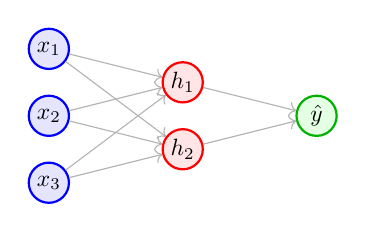
\begin{tikzpicture}[scale=0.85, transform shape,
                neuron/.style={circle, draw, thick, minimum size=0.6cm, inner sep=0pt},
                input/.style={neuron, fill=blue!10, draw=blue},
                hidden/.style={neuron, fill=red!10, draw=red},
                output/.style={neuron, fill=green!10, draw=green!70!black}
            ]
                % Nodes
                \node[input] (i1) at (0, 1) {$x_1$};
                \node[input] (i2) at (0, 0) {$x_2$};
                \node[input] (i3) at (0, -1) {$x_3$};
                
                \node[hidden] (h1) at (2, 0.5) {$h_1$};
                \node[hidden] (h2) at (2, -0.5) {$h_2$};
                
                \node[output] (o) at (4, 0) {$\hat{y}$};
                
                % Connections
                \foreach \i in {1,2,3} \foreach \h in {1,2} \draw[->, gray!60] (i\i) -- (h\h);
                \foreach \h in {1,2} \draw[->, gray!60] (h\h) -- (o);
            \end{tikzpicture}
        \end{column}
    \end{columns}
    \only<2->{\vfill\large\centering $\yhat = f(x_1,x_2,x_3)$}
\end{frame}

% --- SLIDE 2: Agenda Hari Ini (Visual Gambar & Teks) ---
\begin{frame}{\textbf{Data Non-Tabular}}
    Bagaimana jika data kita memiliki struktur \textbf{ruang} (spasial) atau \textbf{waktu} (sekuensial)?
    
    \vspace{0.6cm}
    \begin{columns}[T]
        % Kolom Kiri: CNN / Gambar
        \begin{column}{0.5\textwidth}
            \centering
            \textbf{Gambar}
            
            \vspace{0.4cm}
            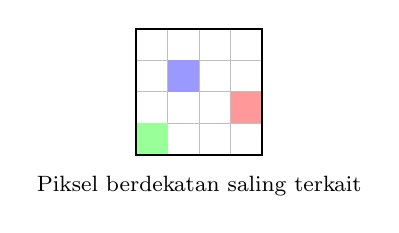
\begin{tikzpicture}[scale=0.8]
                % Kisi piksel sederhana
                \draw[step=0.5cm, gray!50, thin] (0,0) grid (2,2);
                \fill[blue!40] (0.5,1) rectangle (1,1.5);
                \fill[red!40] (1.5,0.5) rectangle (2,1);
                \fill[green!40] (0,0) rectangle (0.5,0.5);
                \draw[thick] (0,0) rectangle (2,2);
                
                \node[font=\footnotesize] at (1, -0.5) {Piksel berdekatan saling terkait};
            \end{tikzpicture}
            
            \vspace{0.4cm}
            \only<2->{\textcolor{blue}{\textbf{Convolutional Neural Networks (CNN)}}}
        \end{column}
        
        % Kolom Kanan: RNN / Teks
        \begin{column}{0.5\textwidth}
            \centering
            \textbf{Teks \& Deret}
            
            \vspace{0.9cm}
            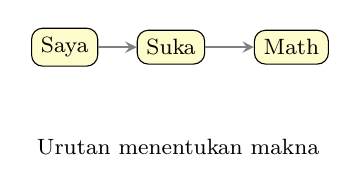
\begin{tikzpicture}[>=stealth, scale=0.9]
                % Blok Teks Sekuensial
                \node[draw, rounded corners, fill=yellow!20, font=\footnotesize] (w1) at (0,-2) {Saya};
                \node[draw, rounded corners, fill=yellow!20, font=\footnotesize] (w2) at (1.5,-2) {Suka};
                \node[draw, rounded corners, fill=yellow!20, font=\footnotesize] (w3) at (3.2,-2) {Math};
                
                \draw[->, thick, gray] (w1) -- (w2);
                \draw[->, thick, gray] (w2) -- (w3);
                
                \node[font=\footnotesize] at (1.6, -3.4) {Urutan menentukan makna};
            \end{tikzpicture}
            
            \vspace{0.4cm}
            \only<3->{\textcolor{red}{\textbf{Recurrent Neural Networks (RNN)}}}
        \end{column}
    \end{columns}
\end{frame}

\subsection{Image Classification}
% --- SLIDE 3: Klasifikasi Gambar (Visualisasi CNN) ---
\begin{frame}{\textbf{Klasifikasi Gambar}}
    \centering
    \vspace{0.3cm}
    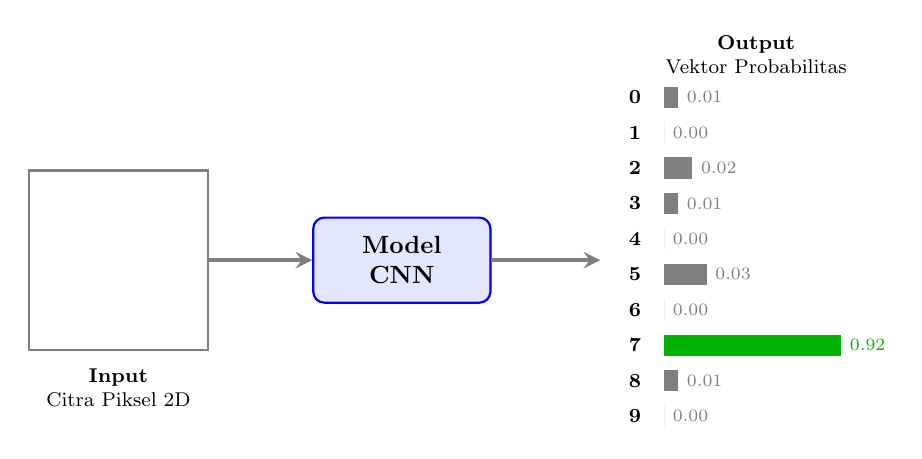
\begin{tikzpicture}[>=stealth, scale=0.9, transform shape]
        
        % 1. Input Image
        % Pastikan file gambar Anda bernama 'mnist_7.png' dan berada di folder yang sama
        \node[inner sep=0pt, draw, thick, gray] (img) at (0, 0) {\exampleimage[2.5cm]{mnist_7.png}};
        \node[font=\footnotesize, align=center] at (0, -1.8) {\textbf{Input}\\Citra Piksel 2D};
        
        % 2. Proses CNN
        \node[draw=blue, fill=blue!10, thick, rounded corners, minimum width=2.5cm, minimum height=1.2cm, align=center] (cnn) at (4, 0) {\textbf{Model}\\\textbf{CNN}};
        
        \draw[->, ultra thick, gray] (img) -- (cnn);
        \draw[->, ultra thick, gray] (cnn) -- (6.8, 0);
        
        % 3. Output Probabilitas (Bar Chart Custom)
        \node[font=\footnotesize, align=center] at (9, 2.9) {\textbf{Output}\\Vektor Probabilitas};
        
        % Looping canggih untuk menggambar 10 bar chart secara otomatis (0-9)
        % Format list: Nilai Teks / Lebar Balok (cm) / Warna
        \foreach \p/\w/\c [count=\i from 0] in {
            0.01/0.2/gray,
            0.00/0.0/gray,
            0.02/0.4/gray,
            0.01/0.2/gray,
            0.00/0.0/gray,
            0.03/0.6/gray,
            0.00/0.0/gray,
            0.92/2.5/green!70!black, % Kelas 7 dibuat sangat menonjol
            0.01/0.2/gray,
            0.00/0.0/gray%
        } {
            % Menghitung koordinat Y agar berjejer rapi ke bawah
            \pgfmathsetmacro{\ypos}{2.3 - \i*0.5}
            
            % Label Kelas (0-9)
            \node[anchor=east, font=\footnotesize\bfseries] at (7.5, \ypos) {\i};
            
            % Visual Bar
            \fill[\c] (7.7, \ypos-0.15) rectangle (7.7+\w, \ypos+0.15);
            
            % Label Probabilitas di ujung bar
            \node[anchor=west, font=\scriptsize, text=\c] at (7.7+\w, \ypos) {\p};
        }
    \end{tikzpicture}
\end{frame}

\subsection{Sentiment Analysis}
% --- SLIDE 4: Klasifikasi Teks (Visualisasi RNN) ---
\begin{frame}{\textbf{Klasifikasi Teks (Analisis Sentimen)}}
    \centering
    \vspace{0.3cm}
    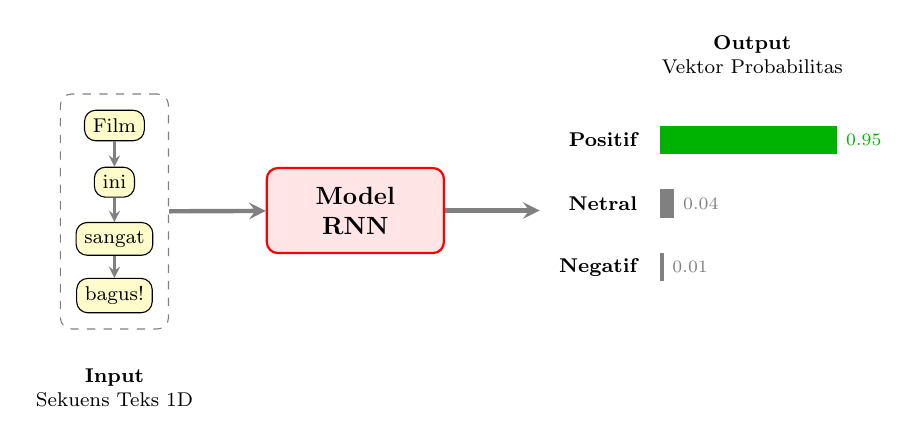
\begin{tikzpicture}[>=stealth, scale=0.9, transform shape]
        
        % 1. Input Teks (Waktu / Sekuensial)
        \node[font=\footnotesize, align=center] at (0, -2.5) {\textbf{Input}\\Sekuens Teks 1D};
        
        % Susunan kata vertikal melambangkan langkah waktu (time steps)
        \node[draw, rounded corners, fill=yellow!20, font=\footnotesize] (w1) at (0, 1.2) {Film};
        \node[draw, rounded corners, fill=yellow!20, font=\footnotesize] (w2) at (0, 0.4) {ini};
        \node[draw, rounded corners, fill=yellow!20, font=\footnotesize] (w3) at (0, -0.4) {sangat};
        \node[draw, rounded corners, fill=yellow!20, font=\footnotesize] (w4) at (0, -1.2) {bagus!};
        
        % Tanda panah urutan waktu
        \draw[->, thick, gray] (w1) -- (w2);
        \draw[->, thick, gray] (w2) -- (w3);
        \draw[->, thick, gray] (w3) -- (w4);
        
        % Membungkus kata-kata menjadi satu kesatuan input
        \node[draw, dashed, gray, rounded corners, fit=(w1) (w4), inner sep=0.2cm] (seq) {};
        
        % 2. Proses RNN / LSTM
        \node[draw=red, fill=red!10, thick, rounded corners, minimum width=2.5cm, minimum height=1.2cm, align=center] (rnn) at (3.4, 0) {\textbf{Model}\\\textbf{RNN}};
        
        % Panah transisi utama
        \draw[->, ultra thick, gray] (seq) -- (rnn);
        \draw[->, ultra thick, gray] (rnn) -- (6, 0);
        
        % 3. Output Probabilitas (Bar Chart Custom)
        \node[font=\footnotesize, align=center] at (9, 2.2) {\textbf{Output}\\Vektor Probabilitas};
        
        % Looping bar chart untuk kelas sentimen
        % Format: Teks / Probabilitas / Lebar / Warna
        \foreach \text/\p/\w/\c [count=\i from 0] in {
            Positif/0.95/2.5/green!70!black, % Kelas dominan
            Netral/0.04/0.2/gray,
            Negatif/0.01/0.05/gray%
        } {
            \pgfmathsetmacro{\ypos}{1 - \i*0.9}
            
            % Label Kelas (Kiri)
            \node[anchor=east, font=\footnotesize\bfseries] at (7.5, \ypos) {\text};
            
            % Visual Bar
            \fill[\c] (7.7, \ypos-0.2) rectangle (7.7+\w, \ypos+0.2);
            
            % Label Probabilitas (Kanan)
            \node[anchor=west, font=\scriptsize, text=\c] at (7.7+\w, \ypos) {\p};
        }
    \end{tikzpicture}
\end{frame}

\section{The Models in Question}
\subsection{Convolutional Neural Networks}
% --- SLIDE 5: Arsitektur Umum CNN ---
\begin{frame}{\textbf{Anatomi Jaringan Saraf Konvolusional (CNN)}}
    \centering
    \vspace{0.2cm}
    
    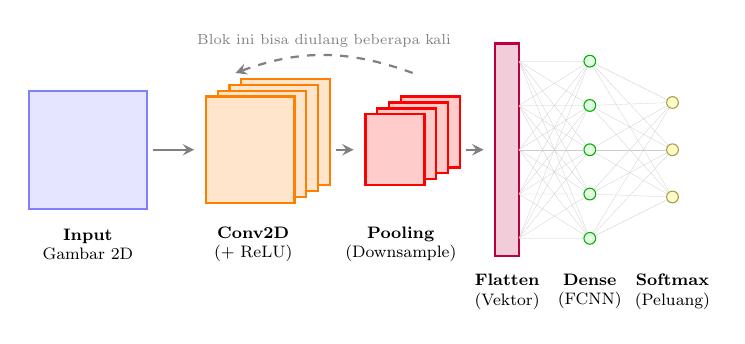
\begin{tikzpicture}[>=stealth, scale=0.75, transform shape]

        % 1. Input Image
        \draw[fill=blue!10, draw=blue!50, thick] (0, -1) rectangle (2, 1);
        \node[font=\footnotesize, align=center] at (1, -1.6) {\textbf{Input}\\Gambar 2D};

        \draw[->, thick, gray] (2.1, 0) -- (2.8, 0);

        % 2. Conv Layer
        \foreach \x in {0.6, 0.4, 0.2, 0} {
            \draw[fill=orange!20, draw=orange, thick] (3+\x, -0.9+\x/2) rectangle (4.5+\x, 0.9+\x/2);
        }
        \node[font=\footnotesize, align=center] at (3.8, -1.6) {\textbf{Conv2D}\\(+ ReLU)};

        % Perbaikan posisi panah agar tidak tertimpa kotak 3D (X-max Conv = 5.1)
        \draw[->, thick, gray] (5.2, 0) -- (5.5, 0);

        % 3. Pooling Layer
        \foreach \x in {0.6, 0.4, 0.2, 0} {
            \draw[fill=red!20, draw=red, thick] (5.7+\x, -0.6+\x/2) rectangle (6.7+\x, 0.6+\x/2);
        }
        \node[font=\footnotesize, align=center] at (6.3, -1.6) {\textbf{Pooling}\\(Downsample)};

        \draw[->, dashed, gray, thick] (6.5, 1.3) to[bend right=20] node[above, font=\scriptsize] {Blok ini bisa diulang beberapa kali} (3.5, 1.3);

        % Perbaikan posisi panah (X-max Pool = 7.3)
        \draw[->, thick, gray] (7.4, 0) -- (7.7, 0);

        % 4. Flatten
        \draw[fill=purple!20, draw=purple, thick] (7.9, -1.8) rectangle (8.3, 1.8);
        \node[font=\footnotesize, align=center] at (8.1, -2.4) {\textbf{Flatten}\\(Vektor)};

        % 5. Dense (Fully Connected)
        % Dideklarasikan dengan index \j agar aman dipanggil tanpa error desimal
        \foreach \y [count=\j] in {-1.5, -0.75, 0, 0.75, 1.5} {
            \node[circle, draw=green!70!black, fill=green!10, inner sep=2pt] (d\j) at (9.5, \y) {};
        }
        \node[font=\footnotesize, align=center] at (9.5, -2.4) {\textbf{Dense}\\(FCNN)};
        
        % Garis jaring (Mesh) dari Flatten ke Dense
        \foreach \fy in {-1.5, -0.75, 0, 0.75, 1.5} {
            \foreach \j in {1, 2, 3, 4, 5} {
                \draw[gray!40, ultra thin] (8.3, \fy) -- (d\j);
            }
        }

        % 6. Softmax (Output)
        \foreach \y [count=\i] in {-0.8, 0, 0.8} {
            \node[circle, draw=yellow!60!black, fill=yellow!20, inner sep=2pt] (s\i) at (10.9, \y) {};
            % Koneksi Dense ke Softmax
            \foreach \j in {1, 2, 3, 4, 5} {
                \draw[gray!40, ultra thin] (d\j) -- (s\i);
            }
        }
        \node[font=\footnotesize, align=center] at (10.9, -2.4) {\textbf{Softmax}\\(Peluang)};

    \end{tikzpicture}

    \vspace{0.3cm}
    \begin{columns}
        \begin{column}{0.48\textwidth}
            \begin{alertblock}{1. Ekstraksi Fitur (Spasial)}
                \textbf{Conv + Pool:} Memindai gambar untuk mencari pola (garis, tekstur), lalu memperkecil resolusinya.
            \end{alertblock}
        \end{column}
        \begin{column}{0.48\textwidth}
            \begin{alertblock}{2. Klasifikasi (Tabular)}
                \textbf{Flatten + Dense:} Meratakan fitur matriks menjadi baris 1D, lalu menebak kelasnya seperti regresi biasa.
            \end{alertblock}
        \end{column}
    \end{columns}
\end{frame}

% --- SLIDE 6: Visualisasi Convolutional Layer ---
\begin{frame}{\textbf{Dari Input ke Output Conv2D}}
    \centering
    \vspace{0.3cm}
    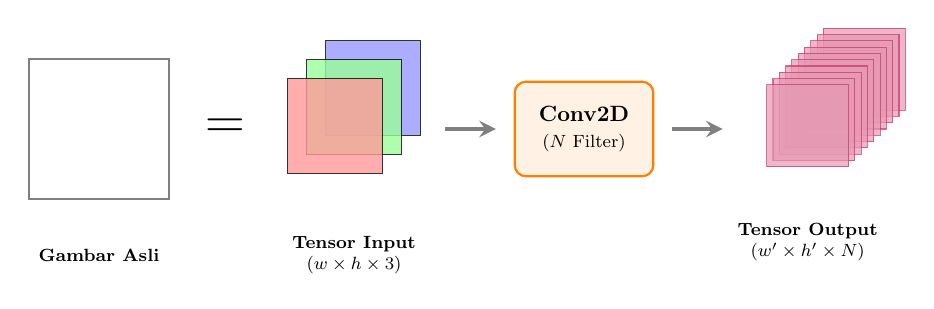
\begin{tikzpicture}[>=stealth, scale=0.8, transform shape]
        
        % 1. Gambar Asli (Placeholder PNG)
        % Silakan ganti 'gambar_input.png' dengan file gambar Anda
        \node[inner sep=0pt, draw, thick, gray] (img) at (0, 0) {\exampleimage[2.2cm]{gambar_input.jpg}};
        \node[font=\footnotesize, align=center] at (0, -2) {\textbf{Gambar Asli}};
        
        % 2. Tanda Sama Dengan
        \node[font=\Huge] (eq) at (2, 0) {$=$};
        
        % 3. Tensor RGB (Input)
        \begin{scope}[shift={(3.0, -0.7)}]
            % Layer Biru, Hijau, Merah ditumpuk manual agar terlihat 3D
            \draw[fill=blue!40, opacity=0.8, draw=black] (0.6,0.6) rectangle (2.1,2.1);
            \draw[fill=green!40, opacity=0.8, draw=black] (0.3,0.3) rectangle (1.8,1.8);
            \draw[fill=red!40, opacity=0.8, draw=black] (0,0) rectangle (1.5,1.5);
            
            \node[font=\footnotesize, align=center] at (1.05, -1.3) {\textbf{Tensor Input}\\$(w \times h \times 3)$};
        \end{scope}
        
        % 4. Panah ke Conv Layer
        \draw[->, ultra thick, gray] (5.5, 0) -- (6.3, 0);
        
        % 5. Kotak Conv Layer
        \node[draw=orange, fill=orange!10, thick, rounded corners, minimum width=2.2cm, minimum height=1.5cm, align=center] (conv) at (7.7, 0) {\textbf{Conv2D}\\\footnotesize ($N$ Filter)};
        
        % 6. Panah ke Output
        \draw[->, ultra thick, gray] (9.1, 0) -- (9.9, 0);
        
        % 7. Tensor Output (Feature Maps)
        \begin{scope}[shift={(10.6, -0.6)}]
            % Menggambar tumpukan tensor output (dimensi w & h lebih kecil, tapi menumpuk tebal ke belakang)
            \foreach \x in {1.8, 1.6, ..., 0} {
                \draw[fill=purple!40, draw=purple!80, opacity=0.7] (\x/2,\x/2) rectangle (1.3+\x/2, 1.3+\x/2);
            }
            \node[font=\footnotesize, align=center] at (0.65, -1.2) {\textbf{Tensor Output}\\$(w' \times h' \times N)$};
        \end{scope}
        
    \end{tikzpicture}
    
    \vspace{0.3cm}
    \begin{columns}
        \begin{column}{0.85\textwidth}
            \begin{itemize}
                \item Gambar direpresentasikan sebagai \textbf{Tensor 3D} (Lebar $\times$ Tinggi $\times$ 3 \textit{Channel} RGB).
                \item \textbf{Convolutional Layer} bertugas mengekstrak fitur menggunakan sejumlah $N$ matriks pemindai (\textit{Filter}).
                \item Hasilnya adalah tensor baru (\textbf{\textit{Feature Maps}}) yang biasanya lebih sempit ukurannya, tetapi lebih tebal lapisannya.
            \end{itemize}
        \end{column}
    \end{columns}
\end{frame}

% --- SLIDE 7: Visualisasi Pooling Layer ---
\begin{frame}{\textbf{Maxpooling untuk Output Conv2D}}
    \centering
    
    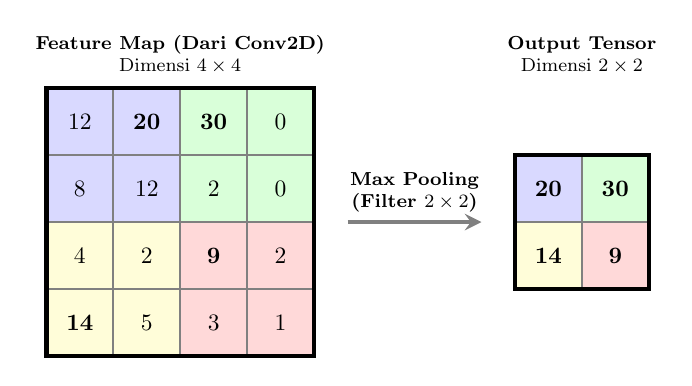
\begin{tikzpicture}[>=stealth, scale=0.85, transform shape]
        
        % --- 1. Matriks Input (4x4) ---
        \begin{scope}[shift={(0,0)}]
            \node[font=\footnotesize, align=center] at (2, 4.5) {\textbf{Feature Map (Dari Conv2D)}\\Dimensi $4 \times 4$};
            
            % Background warna kuadran
            \fill[blue!15] (0, 2) rectangle (2, 4);
            \fill[green!15] (2, 2) rectangle (4, 4);
            \fill[yellow!15] (0, 0) rectangle (2, 2);
            \fill[red!15] (2, 0) rectangle (4, 2);
            
            % Grid
            \draw[step=1cm, thick, gray] (0,0) grid (4,4);
            \draw[ultra thick, black] (0,0) rectangle (4,4);
            
            % Angka di Kuadran Biru (Max: 20)
            \node at (0.5, 3.5) {12}; \node at (1.5, 3.5) {\textbf{20}};
            \node at (0.5, 2.5) {8};  \node at (1.5, 2.5) {12};
            
            % Angka di Kuadran Hijau (Max: 30)
            \node at (2.5, 3.5) {\textbf{30}}; \node at (3.5, 3.5) {0};
            \node at (2.5, 2.5) {2};  \node at (3.5, 2.5) {0};
            
            % Angka di Kuadran Kuning (Max: 14)
            \node at (0.5, 1.5) {4};  \node at (1.5, 1.5) {2};
            \node at (0.5, 0.5) {\textbf{14}}; \node at (1.5, 0.5) {5};
            
            % Angka di Kuadran Merah (Max: 9)
            \node at (2.5, 1.5) {\textbf{9}};  \node at (3.5, 1.5) {2};
            \node at (2.5, 0.5) {3};  \node at (3.5, 0.5) {1};
        \end{scope}
        
        % --- 2. Panah Transisi ---
        \draw[->, ultra thick, gray] (4.5, 2) -- (6.5, 2) 
            node[midway, above, font=\footnotesize\bfseries, align=center, black] {Max Pooling\\(Filter $2 \times 2$)};
            
        % --- 3. Matriks Output (2x2) ---
        \begin{scope}[shift={(7,1)}]
            \node[font=\footnotesize, align=center] at (1, 3.5) {\textbf{Output Tensor}\\Dimensi $2 \times 2$};
            
            % Background warna hasil
            \fill[blue!15] (0, 1) rectangle (1, 2);
            \fill[green!15] (1, 1) rectangle (2, 2);
            \fill[yellow!15] (0, 0) rectangle (1, 1);
            \fill[red!15] (1, 0) rectangle (2, 1);
            
            % Grid
            \draw[step=1cm, thick, gray] (0,0) grid (2,2);
            \draw[ultra thick, black] (0,0) rectangle (2,2);
            
            % Angka Hasil Max Pooling
            \node at (0.5, 1.5) {\textbf{20}};
            \node at (1.5, 1.5) {\textbf{30}};
            \node at (0.5, 0.5) {\textbf{14}};
            \node at (1.5, 0.5) {\textbf{9}};
        \end{scope}
        
    \end{tikzpicture}
    
    \vspace{0.05cm}
    \begin{columns}
        \begin{column}{\textwidth}
            \begin{alertblock}{Mengapa butuh Pooling?}
                \begin{itemize}
                    \item \textbf{Meringankan Komputasi:} Mengurangi resolusi/ukuran matriks secara drastis.
                    \item \textbf{Ekstraksi Fitur Dominan:} Mengambil nilai maksimal (\textit{Max Pooling}) berarti mempertahankan piksel yang memiliki ciri fitur paling kuat.
                \end{itemize}
            \end{alertblock}
        \end{column}
    \end{columns}
\end{frame}

% --- SLIDE 8: Fase Klasifikasi (Flatten, Dense, Softmax) ---
\begin{frame}{\textbf{Fase Klasifikasi: Flatten, Dense, \& Softmax}}
    \centering
    
    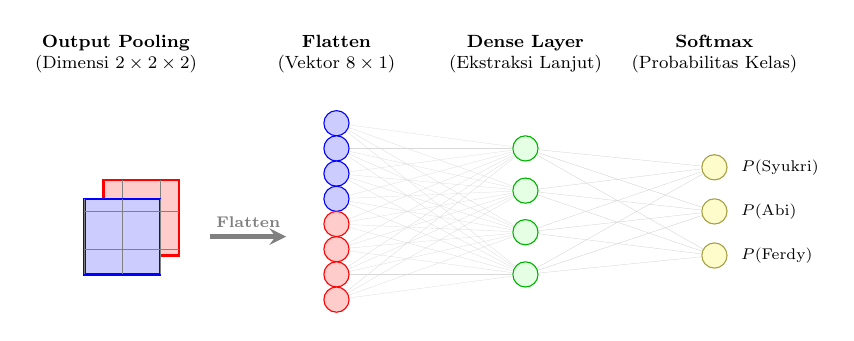
\begin{tikzpicture}[>=stealth, scale=0.8, transform shape]
        
        % 1. Input: Hasil Pooling Terakhir (Bentuk Tensor 3D)
        \begin{scope}[shift={(0,0)}]
            \node[font=\footnotesize, align=center] at (0.5, 2.5) {\textbf{Output Pooling}\\(Dimensi $2 \times 2 \times 2$)};
            % Layer belakang (Channel 2)
            \draw[fill=red!20, draw=red, thick] (0.3, -0.7) rectangle (1.5, 0.5);
            \draw[step=0.6cm, gray, thin] (0.3, -0.7) grid (1.5, 0.5);
            % Layer depan (Channel 1)
            \draw[fill=blue!20, draw=blue, thick] (0, -1) rectangle (1.2, 0.2);
            \draw[step=0.6cm, gray, thin] (0, -1) grid (1.2, 0.2);
        \end{scope}
        
        % 2. Panah Flatten
        \draw[->, ultra thick, gray] (2.0, -0.4) -- (3.2, -0.4) node[midway, above, font=\scriptsize\bfseries] {Flatten};
        
        % 3. Flatten Vector (1D)
        \begin{scope}[shift={(4,0)}]
            \node[font=\footnotesize, align=center] at (0, 2.5) {\textbf{Flatten}\\(Vektor $8 \times 1$)};
            \foreach \y [count=\i] in {1.4, 1.0, 0.6, 0.2, -0.2, -0.6, -1.0, -1.4} {
                % Warnai setengah biru, setengah merah untuk menunjukkan asal channel
                \ifnum\i<5
                    \node[circle, draw=blue, fill=blue!20, inner sep=2pt, minimum size=0.4cm] (f\i) at (0, \y) {};
                \else
                    \node[circle, draw=red, fill=red!20, inner sep=2pt, minimum size=0.4cm] (f\i) at (0, \y) {};
                \fi
            }
        \end{scope}
        
        % 4. Dense Layer (Hidden)
        \begin{scope}[shift={(7,0)}]
            \node[font=\footnotesize, align=center] at (0, 2.5) {\textbf{Dense Layer}\\(Ekstraksi Lanjut)};
            \foreach \y [count=\j] in {1.0, 0.33, -0.33, -1.0} {
                \node[circle, draw=green!70!black, fill=green!10, inner sep=2pt, minimum size=0.4cm] (d\j) at (0, \y) {};
                
                % Koneksi dari Flatten ke Dense (Mesh)
                \foreach \i in {1,...,8} {
                    \draw[gray!30, ultra thin] (f\i) -- (d\j);
                }
            }
        \end{scope}
        
        % 5. Softmax (Output)
        \begin{scope}[shift={(10,0)}]
            \node[font=\footnotesize, align=center] at (0, 2.5) {\textbf{Softmax}\\(Probabilitas Kelas)};
            \foreach \y [count=\k] in {0.7, 0, -0.7} {
                \node[circle, draw=yellow!60!black, fill=yellow!20, inner sep=2pt, minimum size=0.4cm] (s\k) at (0, \y) {};
                
                % Koneksi dari Dense ke Softmax
                \foreach \j in {1,...,4} {
                    \draw[gray!40, ultra thin] (d\j) -- (s\k);
                }
            }
            
            % Label probabilitas di ujung
            \node[anchor=west, font=\scriptsize] at (0.3, 0.7) {$P(\text{Syukri})$};
            \node[anchor=west, font=\scriptsize] at (0.3, 0) {$P(\text{Abi})$};
            \node[anchor=west, font=\scriptsize] at (0.3, -0.7) {$P(\text{Ferdy})$};
        \end{scope}
        
    \end{tikzpicture}
    
    \vspace{0.05cm}
    \begin{columns}
        \begin{column}{\textwidth}
            \begin{alertblock}{Menebak Hasil Akhir}
                \begin{itemize}
                    \item \textbf{Flatten:} Mengubah tensor ruang (3D) yang sudah diringkas menjadi satu deretan angka panjang (1D).
                    \item \textbf{Dense (Fully Connected):} Bekerja layaknya Jaringan Saraf biasa (FCNN).
                    \item \textbf{Softmax:} Memastikan total nilai tebakan di \textit{Output Layer} berjumlah $1$ (atau $100\%$).
                \end{itemize}
            \end{alertblock}
        \end{column}
    \end{columns}
\end{frame}

% --- SLIDE 9: Studi Kasus CIFAR-10 (Visualisasi Arsitektur) ---
\begin{frame}{\textbf{Contoh: Klasifikasi Orang (Who Am I?)}}
    \centering
    \begin{columns}
        
        % --- KOLOM KIRI: Data ---
        \begin{column}{0.5\textwidth}
            \centering
            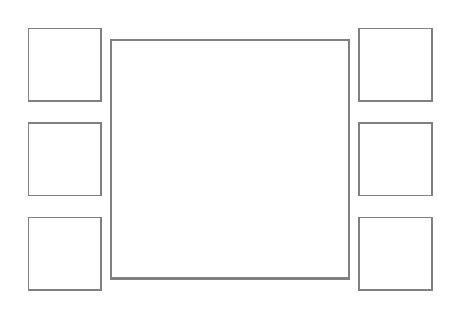
\begin{tikzpicture}
                % 3 Sampel Kecil Kiri
                \node[inner sep=0pt, draw, thin, gray] at (-2.1, 1.2) {\exampleimage[0.9cm]{celeb (1).jpg}};
                \node[inner sep=0pt, draw, thin, gray] at (-2.1, 0) {\exampleimage[0.9cm]{celeb (5).jpg}};
                \node[inner sep=0pt, draw, thin, gray] at (-2.1, -1.2) {\exampleimage[0.9cm]{celeb (3).jpg}};
                
                % Gambar Utama Tengah
                \node[inner sep=0pt, draw, thick, gray] at (0,0) {\exampleimage[3cm]{celeb (2).jpg}};
                
                % 3 Sampel Kecil Kanan
                \node[inner sep=0pt, draw, thin, gray] at (2.1, 1.2) {\exampleimage[0.9cm]{celeb (4).jpg}};
                \node[inner sep=0pt, draw, thin, gray] at (2.1, 0) {\exampleimage[0.9cm]{celeb (6).jpg}};
                \node[inner sep=0pt, draw, thin, gray] at (2.1, -1.2) {\exampleimage[0.9cm]{celeb (7).jpg}};
            \end{tikzpicture}
            
            \vspace{0.2cm}
            \begin{alertblock}{Spesifikasi Data}
                \begin{itemize}
                    \item \textbf{Dimensi:} $32 \times 32$ Piksel
                    \item \textbf{Channel:} 3 (Red, Green, Blue)
                    \item \textbf{Bentuk Input:} $(32, 32, 3)$
                    \item \textbf{Target:} 7 Kategori Objek
                \end{itemize}
            \end{alertblock}
        \end{column}
        
        % --- KOLOM KANAN: Arsitektur Model ---
        \begin{column}{0.4\textwidth}
            \centering
            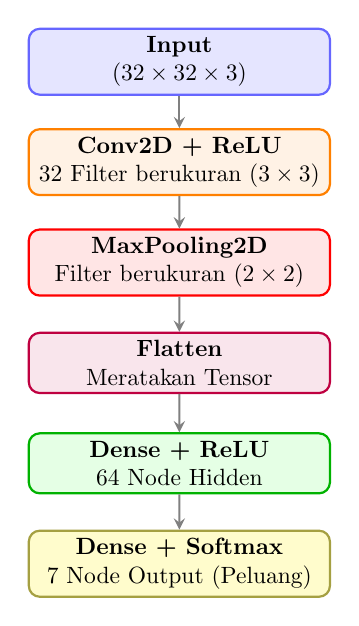
\begin{tikzpicture}[>=stealth, scale=0.85, transform shape,
                box/.style={draw, thick, rounded corners, align=center, minimum width=4.5cm, minimum height=0.7cm},
                arrow/.style={->, thick, gray}
            ]
                % 1. Input
                \node[box, fill=blue!10, draw=blue!60] (input) at (0, 4.5) {\textbf{Input}\\($32 \times 32 \times 3$)};
                
                % 2. Conv2D
                \node[box, fill=orange!10, draw=orange] (conv) at (0, 3) {\textbf{Conv2D + ReLU}\\32 Filter berukuran ($3 \times 3$)};
                
                % 3. Pooling
                \node[box, fill=red!10, draw=red] (pool) at (0, 1.5) {\textbf{MaxPooling2D}\\Filter berukuran ($2 \times 2$)};
                
                % 4. Flatten
                \node[box, fill=purple!10, draw=purple] (flatten) at (0, 0) {\textbf{Flatten}\\Meratakan Tensor};
                
                % 5. Dense 1
                \node[box, fill=green!10, draw=green!70!black] (dense1) at (0, -1.5) {\textbf{Dense + ReLU}\\64 Node Hidden};
                
                % 6. Output (Softmax)
                \node[box, fill=yellow!20, draw=yellow!60!black] (dense2) at (0, -3) {\textbf{Dense + Softmax}\\7 Node Output (Peluang)};
                
                % Garis penghubung
                \draw[arrow] (input) -- (conv);
                \draw[arrow] (conv) -- (pool);
                \draw[arrow] (pool) -- (flatten);
                \draw[arrow] (flatten) -- (dense1);
                \draw[arrow] (dense1) -- (dense2);
                
            \end{tikzpicture}
        \end{column}
        
    \end{columns}
\end{frame}

% --- SLIDE 10: Translasi ke Kode TensorFlow ---
\begin{frame}[fragile]{\textbf{Translasi Arsitektur ke Kode (TensorFlow)}}
    \begin{alertblock}{Membangun Model CNN}
\begin{lstlisting}[language=Python, basicstyle=\ttfamily\scriptsize, keywordstyle=\color{blue}\bfseries, commentstyle=\color{green!50!black}, breaklines=true]
from tensorflow.keras.models import Sequential
from tensorflow.keras.layers import Conv2D, MaxPooling2D, Flatten, Dense

model = Sequential([
    # 1. FASE EKSTRAKSI FITUR (Spasial)
    # Memakai 32 Filter (3x3). Input gambar 32x32 piksel RGB (3 channel)
    Conv2D(32, kernel_size=(3, 3), activation='relu', input_shape=(32, 32, 3)),
    MaxPooling2D(pool_size=(2, 2)),
    
    # 2. FASE TRANSISI
    Flatten(), # Meratakan tensor 3D menjadi vektor 1D
    
    # 3. FASE KLASIFIKASI
    Dense(64, activation='relu'),
    Dense(7, activation='softmax') # 7 orang
])
\end{lstlisting}
    \end{alertblock}
\end{frame}

\subsection{Recurrent Neural Networks}

% --- SLIDE 13: Kelemahan FCNN pada Deret ---
\begin{frame}{\textbf{Tantangan Baru: Data Sekuensial}}
    Misalkan kita memiliki data deret waktu $x = (2, 3, 4)$ dan ingin memprediksi angka selanjutnya $y = (5, 6, 7)$.
    
    \vspace{0.5cm}
    % --- BAGIAN ATAS: DIAGRAM ---
    \begin{center}
        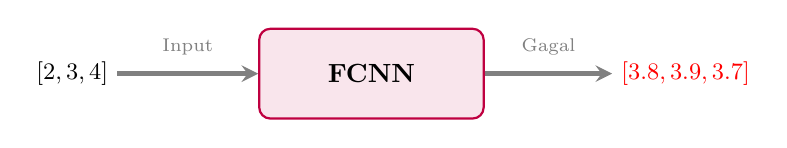
\begin{tikzpicture}[>=stealth, scale=0.95, transform shape]
            \node[draw=purple, fill=purple!10, thick, rounded corners, minimum height=1.2cm, minimum width=3cm] (model) at (0,0) {\textbf{FCNN}};
            
            \node[font=\small] (in) at (-4,0) {$[2, 3, 4]$};
            \node[font=\small, color=red] (out) at (4.2,0) {$[3.8, 3.9, 3.7]$};
            
            \draw[->, ultra thick, gray] (in) -- (model) node[midway, above=0.1cm, font=\scriptsize] {Input};
            \draw[->, ultra thick, gray] (model) -- (out) node[midway, above=0.1cm, font=\scriptsize, align=center] {Gagal};
        \end{tikzpicture}
    \end{center}
    
    \vspace{0.4cm}
    % --- BAGIAN BAWAH: PENJELASAN ---
    \begin{columns}
        \begin{column}{0.95\textwidth}
            \begin{alertblock}{Kegagalan FCNN Biasa}
                \begin{itemize}
                    \item \textbf{Prediksi:} \texttt{[3.85, 3.90, 3.72]}
                    \item \textbf{Alasan:} FCNN memproses seluruh input $2, 3, 4$ secara bersamaan dalam satu lapisan statis. 
                    \item Model ini \textbf{buta terhadap urutan}, ia tidak sadar bahwa angka $4$ muncul setelah angka $3$.
                \end{itemize}
            \end{alertblock}
        \end{column}
    \end{columns}
\end{frame}

% --- SLIDE 14: Konsep RNN & LSTM ---
\begin{frame}{\textbf{Solusi: Recurrent Neural Network (RNN)}}
    RNN memecahkan masalah ini dengan menambahkan \textbf{Memori (\textit{Hidden State}, $h$)} yang dioper ke masa depan.
    
    \centering
    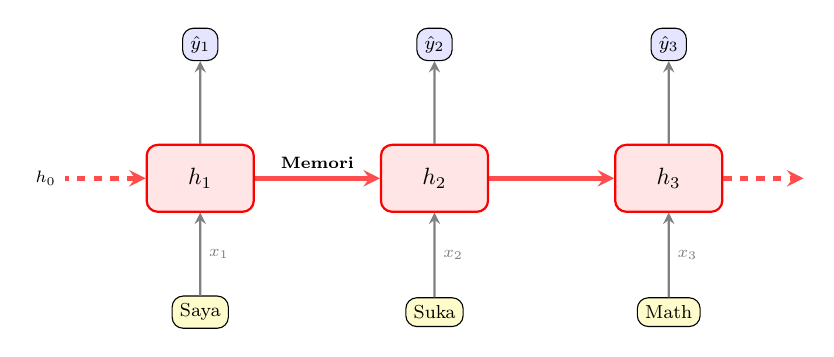
\begin{tikzpicture}[>=stealth, scale=0.85, transform shape]
        % RNN Cells (Unrolled in time)
        \foreach \t/\word [count=\i] in {1/Saya, 2/Suka, 3/Math} {
            % Cell
            \node[draw=red, fill=red!10, thick, rounded corners, minimum width=1.6cm, minimum height=1cm] (rnn\i) at (\i*3.5, 0) {$h_{\t}$};
            % Input
            \node[draw, fill=yellow!20, rounded corners, font=\footnotesize] (x\i) at (\i*3.5, -2) {\word};
            % Output
            \node[draw, fill=blue!10, rounded corners, font=\footnotesize] (y\i) at (\i*3.5, 2) {$\hat{y}_{\t}$};
            
            % Vertical Arrows
            \draw[->, thick, gray] (x\i) -- (rnn\i) node[midway, right, font=\scriptsize] {$x_{\t}$};
            \draw[->, thick, gray] (rnn\i) -- (y\i);
        }
        
        % Horizontal Memory Arrows
        \draw[->, ultra thick, red!70] (rnn1) -- (rnn2) node[midway, above, font=\scriptsize\bfseries, black] {Memori};
        \draw[->, ultra thick, red!70] (rnn2) -- (rnn3);
        
        % In/Out edges
        \draw[<-, ultra thick, red!70, dashed] (rnn1.west) -- ++(-1.2,0) node[left, font=\scriptsize, black] {$h_0$};
        \draw[->, ultra thick, red!70, dashed] (rnn3.east) -- ++(1.2,0);
    \end{tikzpicture}
    
    \begin{alertblock}{Upgrade: LSTM \& GRU}
        RNN pelupa jika kalimatnya terlalu panjang (\textit{Vanishing Gradient}). \textbf{LSTM} (\textit{Long Short-Term Memory}) hadir dengan \textbf{Sistem Gerbang} khusus untuk memilih info mana yang harus diingat jangka panjang dan mana yang dibuang.
    \end{alertblock}
\end{frame}

% --- SLIDE 15: Representasi Teks (Tokenization & Embedding) ---
\begin{frame}{\textbf{Analisis Sentimen: Representasi Teks}}
    Komputer tidak memahami huruf. Bagaimana kita mengubah kalimat menjadi barisan (sekuens) angka untuk RNN?
    
    \begin{center}
        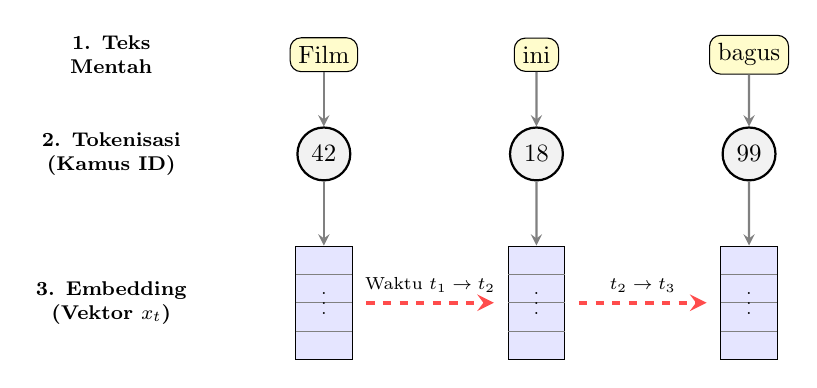
\begin{tikzpicture}[>=stealth, scale=0.9, transform shape]
            % 1. Teks Mentah
            \node[font=\footnotesize\bfseries, align=center] at (-2, 0) {1. Teks\\Mentah};
            \node[draw, rounded corners, fill=yellow!20] (w1) at (1, 0) {Film};
            \node[draw, rounded corners, fill=yellow!20] (w2) at (4, 0) {ini};
            \node[draw, rounded corners, fill=yellow!20] (w3) at (7, 0) {bagus};
            
            % 2. Kamus / Tokenisasi
            \node[font=\footnotesize\bfseries, align=center] at (-2, -1.4) {2. Tokenisasi\\(Kamus ID)};
            \node[draw, circle, thick, fill=gray!10] (id1) at (1, -1.4) {42};
            \node[draw, circle, thick, fill=gray!10] (id2) at (4, -1.4) {18};
            \node[draw, circle, thick, fill=gray!10] (id3) at (7, -1.4) {99};
            
            \draw[->, thick, gray] (w1) -- (id1);
            \draw[->, thick, gray] (w2) -- (id2);
            \draw[->, thick, gray] (w3) -- (id3);
            
            % 3. Embedding / Vektor
            \node[font=\footnotesize\bfseries, align=center] at (-2, -3.5) {3. Embedding\\(Vektor $x_t$)};
            
            % Gambar Vektor (Kotak-kotak kecil ditumpuk)
            \foreach \x/\name in {1/v1, 4/v2, 7/v3} {
                \node[draw, fill=blue!10, minimum width=0.8cm, minimum height=1.6cm] (\name) at (\x, -3.5) {};
                % Garis pemisah isi vektor
                \draw[gray, thin] (\x-0.4, -3.1) -- (\x+0.4, -3.1);
                \draw[gray, thin] (\x-0.4, -3.5) -- (\x+0.4, -3.5);
                \draw[gray, thin] (\x-0.4, -3.9) -- (\x+0.4, -3.9);
                \node[font=\scriptsize] at (\x, -3.4) {$\vdots$};
            }
            
            \draw[->, thick, gray] (id1) -- (v1);
            \draw[->, thick, gray] (id2) -- (v2);
            \draw[->, thick, gray] (id3) -- (v3);
            
            % Panah waktu untuk RNN
            \draw[->, ultra thick, dashed, red!70] (1.6, -3.5) -- (3.4, -3.5) node[midway, above, font=\scriptsize, black] {Waktu $t_1 \rightarrow t_2$};
            \draw[->, ultra thick, dashed, red!70] (4.6, -3.5) -- (6.4, -3.5) node[midway, above, font=\scriptsize, black] {$t_2 \rightarrow t_3$};
        \end{tikzpicture}
    \end{center}
    
    \begin{alertblock}{Persiapan Data}
        \begin{itemize}
            \item Kata diubah menjadi \textbf{ID Numerik} berdasarkan indeks kamus.
            \item ID direntangkan menjadi \textbf{Vektor (\textit{Embedding})} padat agar memiliki makna matematis yang bisa diolah oleh RNN.
        \end{itemize}
    \end{alertblock}
\end{frame}

% --- SLIDE 16: Kode TensorFlow RNN/LSTM ---
\begin{frame}[fragile]{\textbf{Translasi Arsitektur Teks ke Kode}}
    \begin{alertblock}{Membangun Model RNN}
\begin{lstlisting}[language=Python, basicstyle=\ttfamily\scriptsize, keywordstyle=\color{blue}\bfseries, commentstyle=\color{green!50!black}, breaklines=true]
from tensorflow.keras.models import Sequential
from tensorflow.keras.layers import Embedding, LSTM, Dense

model = Sequential([
    # 1. FASE REPRESENTASI KATA
    # input_dim: Jumlah kosa kata di kamus (cth. 10.000 kata teratas)
    # output_dim: Panjang vektor embedding untuk setiap kata (cth. 32)
    Embedding(input_dim=10000, output_dim=32),
    
    # 2. FASE EKSTRAKSI SEKUENSIAL (Waktu)
    # LSTM membaca vektor kata dari awal sampai akhir kalimat
    LSTM(64), # 64 adalah jumlah hidden state / kapasitas memori
    
    # 3. FASE KLASIFIKASI
    # 1 Node dengan Sigmoid misal outputnya hanya Positif (1) / Negatif (0)
    Dense(1, activation='sigmoid')
])
\end{lstlisting}
    \end{alertblock}
    
    \vspace{0.1cm}
    \begin{center}
        \footnotesize \textit{Hanya dengan 3 layer ini, model Anda sudah bisa membaca ulasan film dan merasakan "emosi" dari teks tersebut!}
    \end{center}
\end{frame}

% --- SLIDE 15: Klimaks (Image Captioning) ---
\begin{frame}{\textbf{Puncak Evolusi: \textit{Image Captioning}}}
    Apa jadinya jika kita menggabungkan kejeniusan \textbf{CNN} (Penglihatan) dan \textbf{LSTM} (Bahasa)?
    
    \vspace{0.4cm}
    \centering
    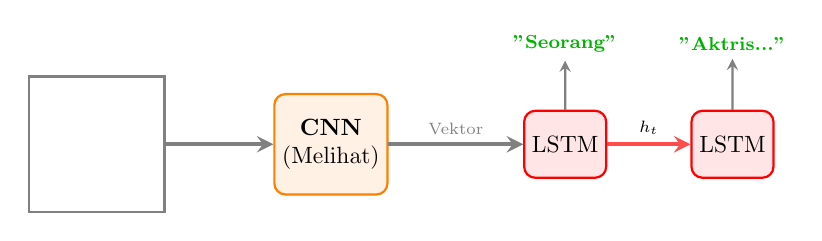
\begin{tikzpicture}[>=stealth, scale=0.85, transform shape]
        % Image (Gunakan kembali file gambar profil Zendaya)
        \node[inner sep=0pt, draw, thick, gray] (img) at (0,0) {\exampleimage[2cm]{celeb (2).jpg}};
        
        % CNN
        \node[draw=orange, fill=orange!10, thick, rounded corners, minimum height=1.5cm, align=center] (cnn) at (3.5,0) {\textbf{CNN}\\(Melihat)};
        
        % LSTM Sequence
        \node[draw=red, fill=red!10, thick, rounded corners, minimum height=1cm] (lstm1) at (7, 0) {LSTM};
        \node[draw=red, fill=red!10, thick, rounded corners, minimum height=1cm] (lstm2) at (9.5, 0) {LSTM};
        
        % Output Words
        \node[font=\footnotesize\bfseries, color=green!70!black] (w1) at (7, 1.5) {"Seorang"};
        \node[font=\footnotesize\bfseries, color=green!70!black] (w2) at (9.5, 1.5) {"Aktris..."};
        
        % Connections
        \draw[->, ultra thick, gray] (img) -- (cnn);
        \draw[->, ultra thick, gray] (cnn) -- (lstm1) node[midway, above, font=\scriptsize] {Vektor};
        \draw[->, ultra thick, red!70] (lstm1) -- (lstm2) node[midway, above, font=\scriptsize, black] {$h_t$};
        
        \draw[->, thick, gray] (lstm1) -- (w1);
        \draw[->, thick, gray] (lstm2) -- (w2);
    \end{tikzpicture}
    
    \vspace{0.4cm}
    \begin{itemize}
        \item \textbf{CNN} memindai foto Zendaya dan merangkumnya menjadi satu vektor padat.
        \item Vektor tersebut disuntikkan ke \textbf{LSTM} sebagai memori awal ($h_0$).
        \item \textbf{LSTM} menerjemahkan memori tersebut dan merangkai kata demi kata untuk mendeskripsikan gambar!
    \end{itemize}
\end{frame}

\section{Praktikum}
\subsection{Demo}
% --- SLIDE Praktikum 1: CNN MNIST ---
\begin{frame}{\textbf{Demo 1: Klasifikasi Digit (MNIST)}}
    
    \begin{columns}[c] % [c] memastikan rata tengah secara vertikal
        
        % --- KOLOM KIRI: Instruksi ---
        \begin{column}{0.55\textwidth}
            \begin{alertblock}{Tugasnya}
                \small 
                \begin{enumerate}
                    \setlength{\itemsep}{0.1cm} 
                    \item \textbf{Muat Data:} Gunakan dataset \texttt{mnist}. Pastikan label menggunakan \texttt{to\_categorical}.
                    \item \textbf{Pre-processing:} Normalisasi piksel (dibagi 255.0), lalu ubah bentuk \textit{array} menjadi tensor 3D: \texttt{(28, 28, 1)}.
                    \item \textbf{Arsitektur Model:} Rangkai balok \texttt{Sequential} mengikuti diagram di kanan.
                    \item \textbf{Pelatihan:} Lakukan \texttt{compile} dan \texttt{fit} (cukup 5 \textit{epochs}).
                    \item \textbf{Inference:} Uji model dengan satu gambar, lalu amati vektor probabilitasnya!
                \end{enumerate}
            \end{alertblock}
        \end{column}
        
        % --- KOLOM KANAN: Cetak Biru Arsitektur ---
        \begin{column}{0.45\textwidth}
            \centering
            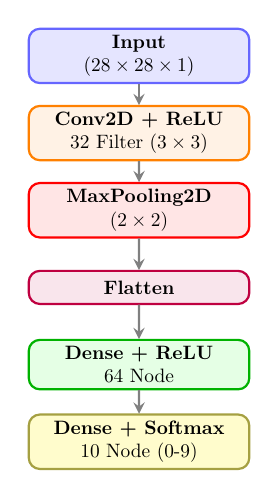
\begin{tikzpicture}[>=stealth, scale=0.7, transform shape,
                box/.style={draw, thick, rounded corners, align=center, minimum width=4cm, minimum height=0.6cm},
                arrow/.style={->, thick, gray}
            ]
                % 1. Input
                \node[box, fill=blue!10, draw=blue!60] (input) at (0, 5) {\textbf{Input}\\($28 \times 28 \times 1$)};
                
                % 2. Conv2D
                \node[box, fill=orange!10, draw=orange] (conv) at (0, 3.6) {\textbf{Conv2D + ReLU}\\32 Filter ($3 \times 3$)};
                
                % 3. Pooling
                \node[box, fill=red!10, draw=red] (pool) at (0, 2.2) {\textbf{MaxPooling2D}\\($2 \times 2$)};
                
                % 4. Flatten
                \node[box, fill=purple!10, draw=purple] (flatten) at (0, 0.8) {\textbf{Flatten}};
                
                % 5. Dense 1
                \node[box, fill=green!10, draw=green!70!black] (dense1) at (0, -0.6) {\textbf{Dense + ReLU}\\64 Node};
                
                % 6. Output (Softmax)
                \node[box, fill=yellow!20, draw=yellow!60!black] (dense2) at (0, -2) {\textbf{Dense + Softmax}\\10 Node (0-9)};
                
                % Garis penghubung
                \draw[arrow] (input) -- (conv);
                \draw[arrow] (conv) -- (pool);
                \draw[arrow] (pool) -- (flatten);
                \draw[arrow] (flatten) -- (dense1);
                \draw[arrow] (dense1) -- (dense2);
                
            \end{tikzpicture}
        \end{column}
        
    \end{columns}
\end{frame}

% --- SLIDE Praktikum 2: RNN IMDB ---
\begin{frame}{\textbf{Demo 2: Analisis Sentimen (IMDB)}}
    
    \begin{columns}[c] 
        
        % --- KOLOM KIRI: Instruksi ---
        \begin{column}{0.55\textwidth}
            \begin{alertblock}{Tugasnya}
                \small 
                \begin{enumerate}
                    \setlength{\itemsep}{0.1cm} 
                    \item \textbf{Muat Data:} Gunakan dataset \texttt{imdb}. Batasi kamus hanya untuk 10.000 kata teratas (\textit{max features}).
                    \item \textbf{Pre-processing:} Gunakan \texttt{pad\_sequences} agar panjang teks seragam (misal \texttt{maxlen=200} kata).
                    \item \textbf{Arsitektur Model:} Rangkai balok \texttt{Sequential} mengikuti diagram di kanan.
                    \item \textbf{Pelatihan:} Lakukan \texttt{compile} (\texttt{binary\_crossentropy}) dan \texttt{fit}.
                    \item \textbf{Inference:} Ambil satu ulasan acak, dekode ID kembali ke teks, lalu lihat apakah model mengenali emosinya!
                \end{enumerate}
            \end{alertblock}
        \end{column}
        
        % --- KOLOM KANAN: Cetak Biru Arsitektur ---
        \begin{column}{0.45\textwidth}
            \centering
            % Karena kotaknya lebih sedikit dari CNN, skala bisa dinaikkan sedikit ke 0.75
            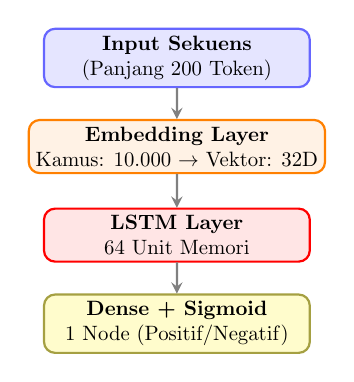
\begin{tikzpicture}[>=stealth, scale=0.75, transform shape,
                box/.style={draw, thick, rounded corners, align=center, minimum width=4.5cm, minimum height=0.6cm},
                arrow/.style={->, thick, gray}
            ]
                % 1. Input
                \node[box, fill=blue!10, draw=blue!60] (input) at (0, 4.5) {\textbf{Input Sekuens}\\(Panjang 200 Token)};
                
                % 2. Embedding
                \node[box, fill=orange!10, draw=orange] (embed) at (0, 3) {\textbf{Embedding Layer}\\Kamus: 10.000 $\rightarrow$ Vektor: 32D};
                
                % 3. LSTM
                \node[box, fill=red!10, draw=red] (lstm) at (0, 1.5) {\textbf{LSTM Layer}\\64 Unit Memori};
                
                % 4. Output (Sigmoid)
                \node[box, fill=yellow!20, draw=yellow!60!black] (dense) at (0, 0) {\textbf{Dense + Sigmoid}\\1 Node (Positif/Negatif)};
                
                % Garis penghubung
                \draw[arrow] (input) -- (embed);
                \draw[arrow] (embed) -- (lstm);
                \draw[arrow] (lstm) -- (dense);
                
            \end{tikzpicture}
        \end{column}
        
    \end{columns}
\end{frame}

\subsection{Exercise}
% --- SLIDE Latihan 1: Fashion MNIST ---
\begin{frame}{\textbf{Latihan 1: Klasifikasi Pakaian (Fashion MNIST)}}
    
    \begin{columns}[c] 
        
        % --- KOLOM KIRI: Instruksi ---
        \begin{column}{0.55\textwidth}
            \begin{alertblock}{Tugasnya}
                \small 
                \begin{enumerate}
                    \setlength{\itemsep}{0.1cm} 
                    \item \textbf{Muat Data:} Gunakan dataset \texttt{fashion\_mnist}. Terdapat 10 kategori pakaian (baju, sepatu, tas, dll). Ubah label dengan \texttt{to\_categorical}.
                    \item \textbf{Pre-processing:} Normalisasi piksel dan ubah bentuk \textit{array} (\textit{reshape}) menjadi tensor 3D: \texttt{(28, 28, 1)}.
                    \item \textbf{Arsitektur Model:} Rangkai balok \texttt{Sequential} seperti di kanan.
                    \item \textbf{Pelatihan:} Gunakan \texttt{categorical\_crossentropy} dan latih selama 5 \textit{epochs}.
                    \item \textbf{Inference:} Uji dengan satu gambar acak dan tebak jenis pakaiannya!
                \end{enumerate}
            \end{alertblock}
        \end{column}
        
        % --- KOLOM KANAN: Cetak Biru Arsitektur ---
        \begin{column}{0.45\textwidth}
            \centering
            % Skala dinaikkan dan minimum width dilebarkan menjadi 5.5cm
            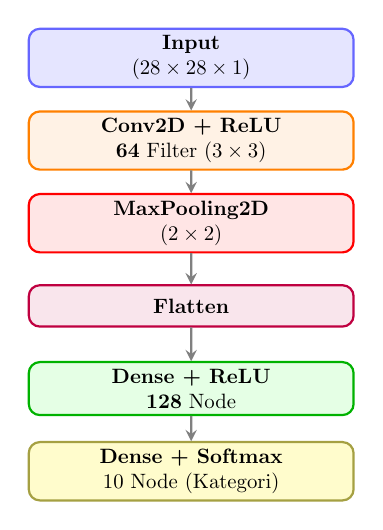
\begin{tikzpicture}[>=stealth, scale=0.75, transform shape,
                box/.style={draw, thick, rounded corners, align=center, minimum width=5.5cm, minimum height=0.7cm},
                arrow/.style={->, thick, gray}
            ]
                % 1. Input
                \node[box, fill=blue!10, draw=blue!60] (input) at (0, 5) {\textbf{Input}\\($28 \times 28 \times 1$)};
                
                % 2. Conv2D
                \node[box, fill=orange!10, draw=orange] (conv) at (0, 3.6) {\textbf{Conv2D + ReLU}\\\textbf{64} Filter ($3 \times 3$)};
                
                % 3. Pooling
                \node[box, fill=red!10, draw=red] (pool) at (0, 2.2) {\textbf{MaxPooling2D}\\($2 \times 2$)};
                
                % 4. Flatten
                \node[box, fill=purple!10, draw=purple] (flatten) at (0, 0.8) {\textbf{Flatten}};
                
                % 5. Dense 1
                \node[box, fill=green!10, draw=green!70!black] (dense1) at (0, -0.6) {\textbf{Dense + ReLU}\\\textbf{128} Node};
                
                % 6. Output (Softmax)
                \node[box, fill=yellow!20, draw=yellow!60!black] (dense2) at (0, -2) {\textbf{Dense + Softmax}\\10 Node (Kategori)};
                
                % Garis penghubung
                \draw[arrow] (input) -- (conv);
                \draw[arrow] (conv) -- (pool);
                \draw[arrow] (pool) -- (flatten);
                \draw[arrow] (flatten) -- (dense1);
                \draw[arrow] (dense1) -- (dense2);
                
            \end{tikzpicture}
        \end{column}
        
    \end{columns}
\end{frame}

% --- SLIDE Latihan 2: Reuters ---
\begin{frame}{\textbf{Latihan 2: Klasifikasi Topik Berita (Reuters)}}
    
    \begin{columns}[c] 
        
        % --- KOLOM KIRI: Instruksi ---
        \begin{column}{0.55\textwidth}
            \begin{alertblock}{Tugasnya}
                \small 
                \begin{enumerate}
                    \setlength{\itemsep}{0.1cm} 
                    \item \textbf{Muat Data:} Gunakan \texttt{reuters} (Kamus: 10.000 kata teratas). Dataset ini berisi berita dengan \textbf{46 topik}.
                    \item \textbf{Pre-processing:} Gunakan \texttt{pad\_sequences} (\texttt{maxlen=200}). Label \textbf{wajib} di-\texttt{to\_categorical}.
                    \item \textbf{Arsitektur Model:} Ikuti bagan di kanan.
                    \item \textbf{Pelatihan:} \texttt{Compile} menggunakan \texttt{categorical\_crossentropy}.
                    \item \textbf{Inference:} Dekode \textit{array} menjadi teks berita, lalu amati prediksi topiknya!
                \end{enumerate}
            \end{alertblock}
        \end{column}
        
        % --- KOLOM KANAN: Cetak Biru Arsitektur ---
        \begin{column}{0.45\textwidth}
            \centering
            % Jarak antar node diatur ulang agar tersebar rata
            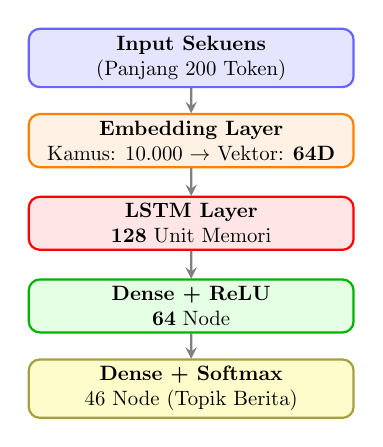
\begin{tikzpicture}[>=stealth, scale=0.75, transform shape,
                box/.style={draw, thick, rounded corners, align=center, minimum width=5.5cm, minimum height=0.7cm},
                arrow/.style={->, thick, gray}
            ]
                % 1. Input
                \node[box, fill=blue!10, draw=blue!60] (input) at (0, 4.5) {\textbf{Input Sekuens}\\(Panjang 200 Token)};
                
                % 2. Embedding
                \node[box, fill=orange!10, draw=orange] (embed) at (0, 3.1) {\textbf{Embedding Layer}\\Kamus: 10.000 $\rightarrow$ Vektor: \textbf{64D}};
                
                % 3. LSTM
                \node[box, fill=red!10, draw=red] (lstm) at (0, 1.7) {\textbf{LSTM Layer}\\\textbf{128} Unit Memori};
                
                % 4. Dense Hidden
                \node[box, fill=green!10, draw=green!70!black] (dense1) at (0, 0.3) {\textbf{Dense + ReLU}\\\textbf{64} Node};
                
                % 5. Output (Softmax)
                \node[box, fill=yellow!20, draw=yellow!60!black] (dense2) at (0, -1.1) {\textbf{Dense + Softmax}\\46 Node (Topik Berita)};
                
                % Garis penghubung
                \draw[arrow] (input) -- (embed);
                \draw[arrow] (embed) -- (lstm);
                \draw[arrow] (lstm) -- (dense1);
                \draw[arrow] (dense1) -- (dense2);
                
            \end{tikzpicture}
        \end{column}
        
    \end{columns}
\end{frame}
\end{document}